\documentclass[11pt]{book}
\usepackage{hyperref}
\usepackage{amsfonts}
\usepackage{amsmath}
\usepackage[utf8]{inputenc}
\usepackage[T1]{fontenc}
\usepackage{float}
\usepackage{fixltx2e}
\usepackage[italian]{babel}
\usepackage{graphicx}

\title{Appunti di Ricerca Operativa}
\author{Fabio Viola}
\date{}

\hyphenation{mi-ni-miz-za-re}

\setcounter{chapter}{1}

\begin{document}

\chapter{Programmazione matematica}

\scriptsize
{\bf Slide}:
\href{http://www.or.deis.unibo.it/staff_pages/martello/Chapter2.zip}{Mathematical
Programming}
\normalsize
\vspace{20pt}

Un {\bf problema di ottimizzazione} \`e un problema nel quale bisogna
{\bf minimizzare} o {\bf massimizzare} una funzione detta
rispettivamente {\bf funzione costo} o {\bf funzione profitto}. Tale
funzione pu\`o essere dunque espressa come: $\underset{x \in
  F}{min}\phantom{a}\varphi(x)$ oppure $\underset{x \in
  F}{max}\phantom{a}\varphi(x)$.

In questa funzione $x$ \`e un vettore di {\bf variabili decisionali},
un elemento di $\mathbb{R}^n$ che possiamo scrivere evidenziando le
sue componenti come: $x = (x_1,x_2,\dots,x_n) \in \mathbb{R}^n$.  In
$\mathbb{R}^n$ troviamo anche l'insieme $F$ delle {\bf soluzioni
  ammissibili}. La {\bf funzione obiettivo} $\varphi:F\rightarrow R$
cerca un punto $x^* \in \mathbb{R}$ che possa costituire un {\bf
  ottimo globale} e che dia dunque il minimo (o il massimo) cercato.
Trovare il minimo significa trovare $x^* \in
F\phantom{a}t.c.\phantom{a}\varphi(x^*) \leq
\varphi(x)\phantom{a}\forall x \in F$ (per il massimo vale chiaramente
la stessa relazione con il segno di $\geq$). La funzione obiettivo,
come precedentemente detto, costituisce solitamente o un problema di
massimizzazione o di minimizzazione. Possiam passare da uno all'altro
con la relazione: $max \varphi(x) = -min(-\varphi(x))$.

La {\bf regione ammissibile {\em F}} viene normalmente definita
tramite disequazioni ($g_i(x)$) e/o equazioni ($h_j(x)$). \`E proprio
su tali vincoli, oltre che sulla funzione $\varphi$, che si basano le
nostre classificazioni sui problemi:

\begin{itemize}
  
\item {\bf programmazione non lineare}: se $g_i$, $h_j$ e $\varphi$
  sono {\em funzioni generali}. In generale la funzione potrebbe non
  essere continua, oppure lo spazio delle soluzioni potrebbe essere
  vuoto o anche questo non continuo. In questo caso conosciamo
  soltanto algoritmi non efficienti che possono trovare l'ottimo
  globale solo per problemi di piccole dimensioni. Per problemi pi\`u
  grandi \`e possibile trovare ottimi locali (ne possiamo avere pi\`u
  di uno);

\item {\bf programmazione convessa}: se $\varphi$ e $g_i$ sono {\bf
  convesse} (vedremo a breve cosa si intende) e $h_j$ \`e {\bf
  lineare}. Anche in questi problemi abbiamo solo algoritmi che
  operano su piccoli problemi trovando ottimi locali, {\bf ma} in
  questo caso gli ottimi locali sono anche ottimi globali;

\item {\bf programmazione lineare}: se sia $\varphi$ che i vincoli
  sono lineari. Per questi problemi abbiamo a disposizione un
  algoritmo molto efficiente, il {\bf metodo del simplesso}, che trova
  facilmente l'ottimo globale per problemi di qualsiasi dimensione.

\end{itemize}

Un altra definizione di problema che possiamo dare \`e $(F, d)$ dove
$F$ \`e l'insieme delle soluzioni ammissibili e $d$ \`e la {\bf
  funzione costo} $d:\phantom{a}F\rightarrow R^1$.

%% %% $\[\left\{
%% %% \begin{array}{l l l}
%% %%   (F,d)\\
%% %%   F=\{x \in \mathbb{R}^n : Ax = b, x \geq 0\}\\
%% %%  
%% %% \end{array} \right\]$

%% \begin{equation}
%%  \left.\begin{aligned} min\phantom{a}c'x\\ Ax=b\\ x\geq 0
%%  \end{aligned}
%%  \right\}\Leftrightarrow \left\{\begin{aligned} (F,d)\\ F=\{x\in
%%  \mathbb{R}^n : Ax = b, x \geq 0\}\\ d:x \rightarrow c'x
%%  \end{aligned}
%%  \right.
%% \end{equation} 

Un'altra formulazione che possiamo fare \`e $min\phantom{a}c'x$,
$Ax=b$. In questa formulazione $c'$ \`e il vettore dei coefficienti
della funzione obiettivo, $x$ \`e un vettore colonna contenente le
incognite, $A$ \`e una matice di {\em m} righe ed {\em n} colonne
contenente i coefficienti dei vincoli, $b$ \`e un vettore colonna
contenente i termini noti. Notiamo che $c'$ \`e un vettore ottenuto
con la trasposizione del vettore $c$. Alcune definizioni che ci
torneranno utili sono:

\begin{itemize}
\item $A_j$: colonna della matrice;
\item ${a'}_i$: riga della matrice;
\item $det(A)$: determinante della matrice;
\item $a_{ij}$: elemento situato alla riga $i$ e colonna $j$ della
  matrice.
\end{itemize}

Proseguiamo con le definizioni. Introduciamo ora il concetto di {\bf
  intorno}. Definito $2^F$ l'insieme di tutti i sottoinsiemi di $F$,
potremmo, in maniera molto generale, definire l'intorno come una
funzione $N:F\rightarrow2^F$, cio\`e come una funzione che associa ad
un punto di $F$ un sottoinsieme di $2^F$. In questo caso il
sottoinsieme di destinazione potrebbe essere qualunque, quindi la
definizione \`e molto vaga. Per una definizione pi\`u precisa
introduciamo dunque l'{\bf intorno euclideo}: si tratta dell'insieme
di punti che non dista pi\`u di $\varepsilon$ da un punto $x$. Pi\`u
formalmente: $x \in F:\phantom{a}N_{\varepsilon}(x)=\{y \in
F:\|y-x\|\leq\varepsilon\}$

Dato un problema $(F,d)$ ed un intorno $N$, $f\in F$ \`e un {\bf
  ottimo locale} di $N$ se $d(f) \leq d(g)\phantom{a}\forall g \in
N(f)$. $N$ si dice {\bf esatto} se $f\in F$ ottimo locale ad $N$
implica che $f$ \`e un ottimo globale.

%% TODO esempio?! slide 7

A questo punto \`e giunto il momento di introdurre il concetto di {\bf
  convessit\`a}.  Dati due elementi {\em x} e {\em y} di
$\mathbb{R}^n$, si dice {\bf combinazione convessa} di {\em x} e {\em
  y} qualunque $z \in \mathbb{R}^n$ definita da: $z = \lambda x +
(1-\lambda)y \text{ con } \lambda \in
\mathbb{R}^1,\phantom{a}0\leq\lambda\leq 1$. In pratica \`e ogni punto
sul segmento che unisce {\em x} e {\em y}.

Definiamo {\bf insieme convesso} un insieme $S \subset C$ tale che:
$\forall x,y \in
S,\phantom{a}\forall\lambda\phantom{a}(0\leq\lambda\leq 1), z =
\lambda x + (1-\lambda)y \in S$. Un insieme {\em S} \`e dunque
convesso se ogni punto al suo interno pu\`o essere unito con un
segmento i cui punti siano ancora tutti appartenenti ad $S$.

\begin{figure}[h!]
  \centering
  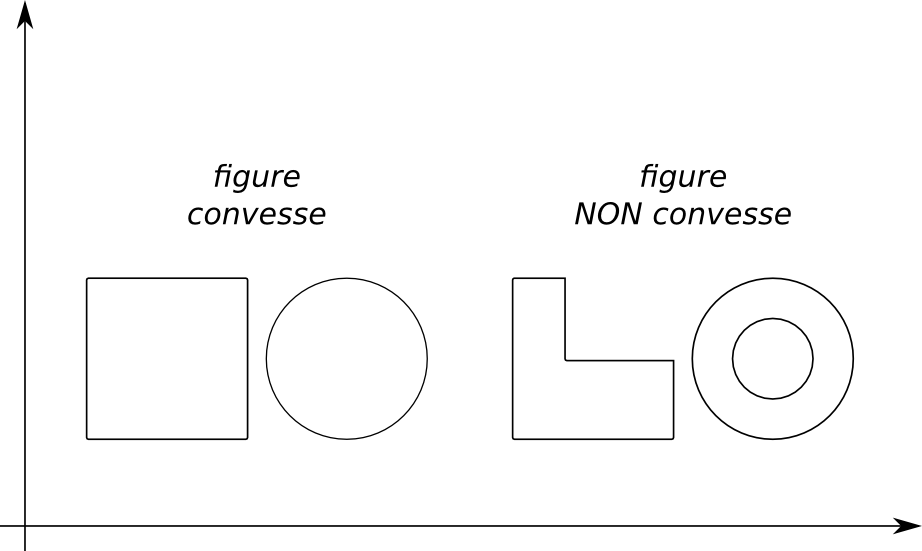
\includegraphics[width=0.7\textwidth]{images/convessita.png}
  \caption{Figure convesse e non}
  \label{convessita}
\end{figure}

Seguono alcune semplici propriet\`a:

\begin{itemize}
\item {\bf Propriet\`a 0}: $\mathbb{R}^n$ \`e convesso;
\item {\bf Propriet\`a 1}: dati {\em n} set convessi, la loro
  intersezione \`e convessa.
  {\bf \underline{Dimostrazione}}: $x, y \in \cap S_i \Rightarrow x,y
  \in S_i \forall i \Rightarrow z \in S_i \forall i \Rightarrow z \in
  \cup S_i$.
  La dimostrazione prende due punti {\em x} e {\em y} contenuti
  nell'intersezione di {\em n} set convessi. Trovandosi
  nell'intersezione, appartengono a tutti gli {\em n} insiemi
  considerati e quindi {\em z} si trover\`a in tutti gli insiemi e
  dunque anche nell'intersezione e dunque tale intersezione \`e
  convessa.
\end{itemize}

Dato un sottoinsieme $S \subset \mathbb{R}^n$ convesso, la funzione
costo $c:S\rightarrow \mathbb{R}^1$ \`e convessa in $S$ se: $\forall
x,y \in S, \forall \lambda(0 \leq \lambda \leq 1), c(\lambda x +
(1-\lambda)y) \leq \lambda c(x) + (1-\lambda)c(y)$. A parole possiam
dire che una funzione \`e convessa in $S$ se presi due punti
qualunque, il costo in qualunque punto del grafico che li unisce \`e
inferiore alla somma dei costi in {\em x} e {\em y}, ancora pi\`u
facilmente possiamo dire che \`e convessa se la funzione pende al di
sotto della linea che unisce i due punti.

%% TODO figura slide 8 (9 di 12)

\begin{itemize}
\item {\bf Propriet\`a 2}Data una funzione $c(x)$ convessa in $S$
  convesso, $\forall t S_t = \{x\in S : c(x) \leq t\}$ \`e convesso.
    
    {\bf \underline{Dimostrazione}}: dati $x,y \in S_t, \lambda x +
    (1-\lambda)y\in S$ e sapendo che $c(\lambda x+ (1-\lambda)y) \leq
    \lambda c(x) + (1-\lambda)c(y) \leq \lambda t + (1-\lambda)t = t
    \Rightarrow \lambda x+ (1-\lambda)y \in S_t$.
\end{itemize}

Avendo definito una funzione convessa, possiamo definire cosa si
intende con {\bf funzione concava}: una funzione \`e concava se la sua
inversa \`e convessa. Una funzione {\bf lineare} \`e sia concava che
convessa.


\section{Programmazione convessa}

Analizziamo il problema di minimizzare una funzione convessa in un set
convesso:

{\bf \underline{Teorema}}: dato un problema $(F,c)$ con $F \subset
\mathbb{R}^n$ convesso e dato {\em c} convesso in {\em F}, il vicinato
$N\varepsilon (x) = \{y\in F :\|x-y\|\leq \varepsilon\}$ \`e esatto
$\forall \varepsilon > 0$.

{\bf \underline{Dimostrazione}}: consideriamo {\em x} ottimo locale
rispetto a $N_{\varepsilon}$ e $y \in F$. Prendiamo $z = \lambda x +
(1-\lambda)y \in N_{\varepsilon}(x)$ con $\lambda$ molto prossimo a 1
(e quindi molto vicino a {\em x}). Avremo $c(z) = c(\lambda x +
(1-\lambda)y) \leq \lambda c(x) + (1-\lambda)c(y) \Rightarrow c(y)
\geq \frac{c(z)-\lambda c(x)}{1-\lambda}$. Inoltre $z \in
N_{\varepsilon}(x) \Rightarrow c(z) \geq c(x) \Rightarrow c(y) \geq
\frac{c(x)-\lambda c(x)}{1-\lambda} = c(x)$

\vspace{20pt}

$(F,c)$ \`e un programma di programmazione convessa ({\bf CP}) se {\em
  c} \`e convessa, $F \subset \mathbb{R}^n$ \`e definito da
disequazioni concave $g_i(x)\geq 0\phantom{a}(i=1,\dots,q)$. Un
vincolo espresso come equazione lineare $h_j(x)=0$ pu\`o essere
rimpiazzato con due disequazioni concave $h_j(x)\geq 0$ e $h_j(x)\leq
0$.

{\bf Propriet\`a}: in un programma di programmazione convessa {\em F}
\`e convessa, quindi un ottimo locale (secondo la definizione di
{\em intorno euclideo}) \`e anche un ottimo globale.

\end{document}
